\subsection*{Регуляризация: зачем и как}
Веса модели могут принимать любые значения. Считаем логичным, 
что чем больше вес у определённого признака, тем этот признак 
важнее для предсказания. И наоборот, чем вес меньше, тем 
наименее полезен. Звучит логично, но иногда бывают ситуации, когда 
слишком большие или слишком малые веса приводят к неожиданному поведению
модели. Посмотрите на следующее изображение:
\begin{figure}[H]
    \centering
    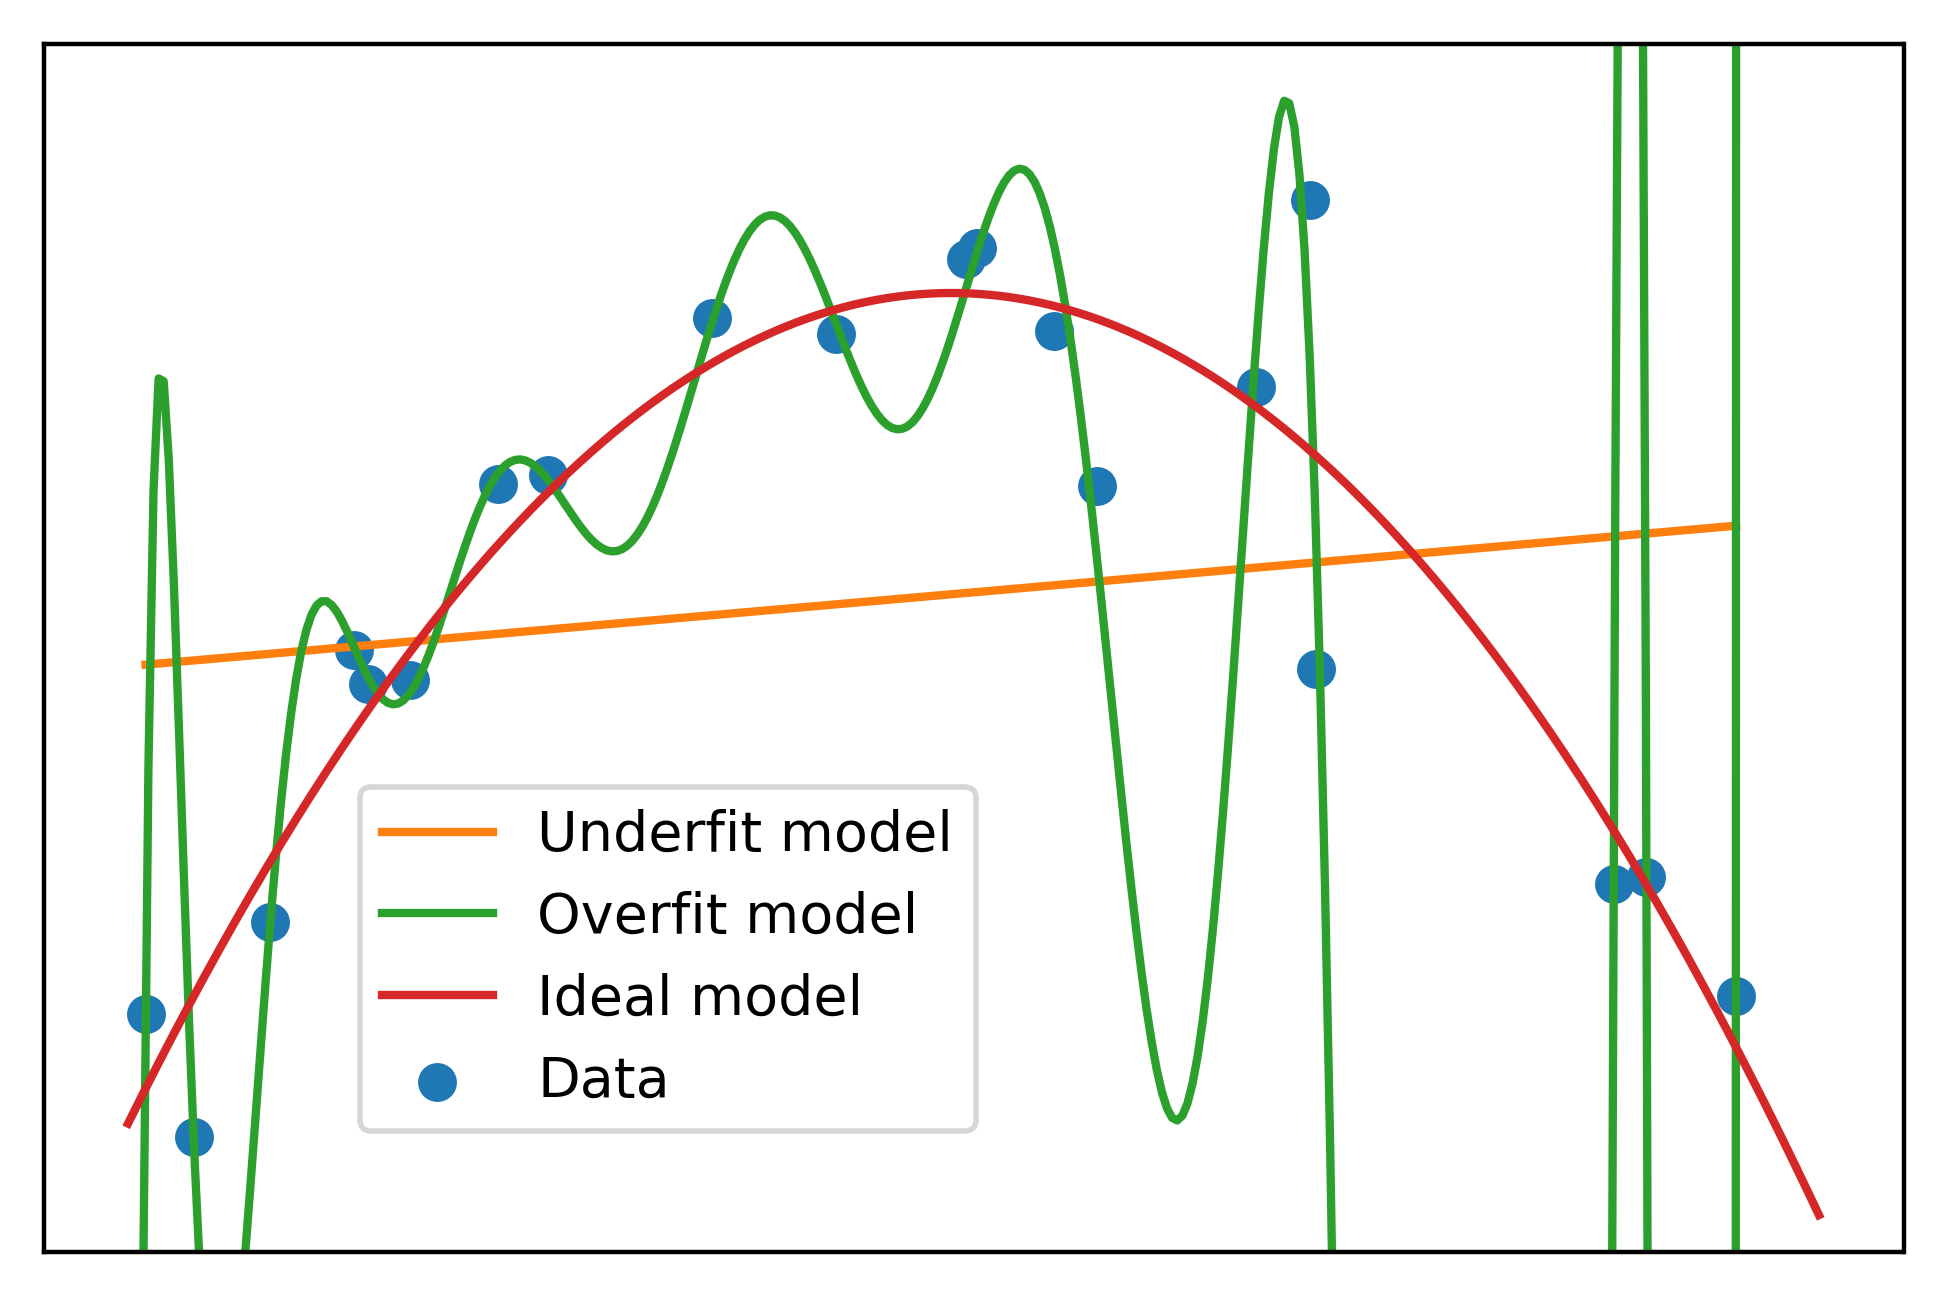
\includegraphics[width=0.75\linewidth]{media/under_cool_overfitting.png}
    \caption{Поведение модели в зависимости от весов}
\end{figure}

Красная модель является в некотором смысле идеальной. В каждой задаче 
мы предполагаем, что существует функция, которая идеально описывает 
данные, и наша задача "--- как можно ближе восстановить эту функцию.

Оранжевая модель не справляется с задачей описания представленных 
данных. Не вдаваясь в подробности, такой случай называется 
\textit{недообучением} (\texttt{underfitting}). Модель так 
и не научилась описывать данные "--- это может быть связанно с, например,
маленьким количеством представленных данных.

Зелёная модель слишком хорошо справляется с обучающими примерами, 
буквально проходя через каждую из точек. Проблема заключается в том,
что при поступлении новых данных, эта модель, многовероятно, будет 
предсказывать очень плохо. А зачем нам модель, если она не сможет 
предсказывать что"=то на новых данных? Такое поведение модели называется \textit{переобучением} \texttt{overfitting}, и это является наиболее насущной проблемой, с 
которой нужно бороться в любом случае.

Есть чисто эмпирическое наблюдение, которое заключается в том, что 
если у модели по модулю большие веса "--- это означает, что скорее всего
она переобучена.

Мы рассмотрим метод, который в литературе обычно называют 
\texttt{weight decay} (уменьшение весов), и его идея донельзя проста:
давайте просто к функционалу потерь приблавлять эти же веса, с некоторым
коэффициентом $\alpha$. Этот коэффициент будет выражать степень 
силы регуляризации. Для \texttt{MSE}:
\[
\frac{1}{\ell}\sum_{i=1}^\ell (a(x_i) - y_i)^2 + \alpha||w||_1
\]
$||w||_1$ "--- это умное обозначение всех элементов вектора. Это называют
$L_1$ регуляризацией.

Теперь нам надо минимизировать не только отклонение предсказания от 
ответа, но ещё и сумму весов, домноженную на какой"=то коэффициент
($\alpha \in [0,1]$), и нашей модели теперь непозволительно делать 
какие"=то большие значения весов.

Есть ещё один вид регуляризации. Прежде чем задаваться вопросами 
<<а зачем>>, давайте обсудим её. Идея та же, но теперь 
делаем не просто сумму, а сумму квадратов весов:
\[
\frac{1}{\ell}\sum_{i=1}^\ell (a(x_i) - y_i)^2 + \alpha||w||_2^2
\]
Это же чудо называется $L_2$ регуляризацей. Интуитивно, чем больше
вес "--- тем сильнее штраф.

Ну и теперь осталось обсудить самое главное "--- зачем нам 2 
типа регуляризации?

Дело в том, что $L_1$ обладает интересной способностью \textit{занулять}
некоторые веса, а соответственно и признаки. Существует множество 
способов описать такое поведение, но давайте взглянем на наиболее
интуитивно понятное.

Прежде чем приступать, надо объяснить, что такое линии уровня.
Представьте себе сложную трёхмерную функцию, на которую мы смотрим
сверху так, чтобы она выглядела как двумерная "--- это и есть линии 
уровня. С помощью такого приёма мы можем проецировать многомерные 
функции в пространство меньшей размерности. Взглянем на следующее 
изображение:
\begin{figure}[H]
    \centering
    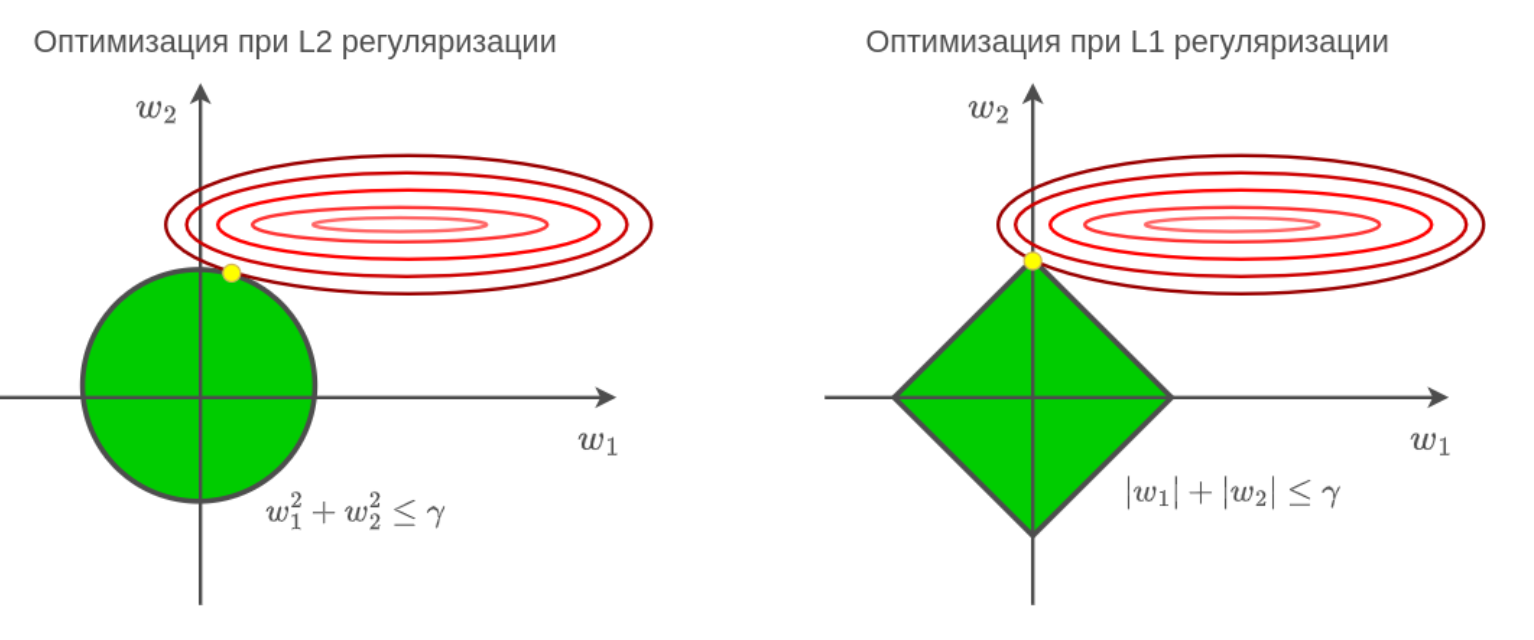
\includegraphics[width=1\linewidth]{media/l1_zeroing.png}
\end{figure}

Красная проекция "--- это линии уровня для \texttt{MSE}. Рассмотрим 
подробнее левое изображение. Зелёный график "--- это интерпретация
$L_2$ нормы для двух весов. Действительно, получится $w_1^2 + w_2^2$,
что есть уравнение круга с центром в точке $(0, 0)$. Пересечение круга 
с линиями уровнями означает, что \texttt{MSE} достигает своего 
минимального значения именно в этой точке пересечения. Заметим, что при
этом вес ненулевой.

Теперь рассмотрим $L_1$ = $|w_1| + |w_2|$. Это есть уравнение ромба, 
что мы и видим на рисунке справа. Пересечение в большинстве случаев
происходит в угловой точке ромба, где один из весов (в данном случае
$w_2$) равняется $0$. 

Выходит, что в некоторых ситуациях, с точки зрения $L_1$ оптимально 
будет занулять некоторые веса.